\documentclass[review]{elsarticle}

\usepackage{lineno,hyperref}

\modulolinenumbers[5]

\journal{Petroleum Science}

%%%%%%%%%%%%%%%%%%%%%%%
%% Elsevier bibliography styles
%%%%%%%%%%%%%%%%%%%%%%%
%% To change the style, put a % in front of the second line of the current style and
%% remove the % from the second line of the style you would like to use.
%%%%%%%%%%%%%%%%%%%%%%%

%% Numbered
%\bibliographystyle{model1-num-names}

%% Numbered without titles
%\bibliographystyle{model1a-num-names}

%% Harvard
%\bibliographystyle{model2-names.bst}\biboptions{authoryear}

%% Vancouver numbered
%\usepackage{numcompress}\bibliographystyle{model3-num-names}

%% Vancouver name/year
%\usepackage{numcompress}\bibliographystyle{model4-names}\biboptions{authoryear}

%% APA style
%\bibliographystyle{model5-names}\biboptions{authoryear}

%% AMA style
%\usepackage{numcompress}\bibliographystyle{model6-num-names}

%% `Elsevier LaTeX' style
\bibliographystyle{elsarticle-num}
%%%%%%%%%%%%%%%%%%%%%%%

\begin{document}

\begin{frontmatter}

%\title{Elsevier \LaTeX\ template\tnoteref{mytitlenote}}
\title{Further evidence of unstable reverse polarity geomagnetic field across the
Olduvai subchron: paleomagnetic and multispecimen paleointensity study
on Khertvisi lava flows (Lesser Caucasus)}

%% Group authors per affiliation:
\author[a]{Avto Goguitchaichvili}
\author[a]{Juan Morales}
\author[b]{Goga Vashakidze}
\author[c]{Manuel Calvo-Rathert}
\author[d]{Vladimir A.Lebedev}
\author[e]{Vadim Kravchinsky}
\author[a]{Miguel Cervanas-Solano}
\author[a]{Daniel Sebastian Reyes}

\address[a]{Laboratorio Interinstitucional de Magnetismo Natural, Instituto de Geofísica, UNAM – Campus Morelia, M\'{e}xico}
\address[b]{I. Javakhishvili Tbilisi State University, Tbilisi, Georgia}
\address[c]{Departamento de Física, EPS Campus Rio Vena – Universidad de Burgos, 09006 Burgos, Spain}
\address[d]{Institute of Geology of Ore Deposits, Petrography, Mineralogy and Geochemistry, Russian Academy of Sciences (IGEM RAS), Moscow, Russia}
\address[e]{Geophysics, Department of Physics, University of Alberta, Edmonton, Alberta T6G2E1, Canada}
%\fntext[myfootnote]{Since 1880.}

%% or include affiliations in footnotes:
%\author[mysecondaryaddress]{\corref{mycorrespondingauthor}}
\cortext[mycorrespondingauthor]{Corresponding author}
\ead{}

\begin{abstract}
Goguitchaichvili et al. (Physics of the Earth and Planetary Interiors, doi.org/ 10.1016/j.pepi.2020.106641, 2021) reported a detailed rock-magnetic and paleointensity study of a Lesser Caucasus lava sequence comprised between 1.93 ± 0.09 and 1.78 ± 0.11 Ma. Reverse polarity magnetization determined for 20 consecutive lava flows permitted to suggest that the Olduvai subchron is probably disrupted by a short reverse-polarity episode. No paleointensity was obtained because of thermally unstable samples. Here, we report a detailed rock-magnetic, paleomagnetic, and multispecimen parallel differential pTRM absolute paleointensities performed on the nearby parallel Khertvisi lava succession. New isotopic age determinations indicate that the lavas of the Khertvisi section erupted in the Early Pleistocene, at the boundary of Gelasian and Calabrian ages in a time span of 1.88 ± 0.10 to 1.71 ± 0.12 Ma. All lava flows yielded well-defined reverse polarity magnetization with site mean directions.e values of the virtual geomagnetic pole (VGP) scatter parameters indicate that the studied sequence was formed during a very short time, most probably insufficient to average paleosecular variation. The multispecimen methodology provided a relatively low paleointensity for most analyzed lava flows, comparable to the transitional field intensity in Georgia during the Bruhnes and Matuyama chrons. These results definitively confirm a rather unstable, reverse polarity geomagnetic field regime across the Olduvai normal superchron. Thus, we propose to consider the Khertvisi section as the firm, volcanic evidence of Olduvai’s short-lived geomagnetic event.
\end{abstract}

\begin{keyword}
\texttt Paleomagnetism \sep Multi-specimen paleointensity \sep Olduva \sep Caucasus
\MSC[2010] 00-01\sep  99-00
\end{keyword}

\end{frontmatter}

\linenumbers
%%/////////////////////////////////////////////////////////////////////////////////////%%
%%/////////////////////////////////////////////////////////////////////////////////////%%
%%/////////////////////////////////////////////////////////////////////////////////////%%
\section{Introduction}

\paragraph {} Geomagnetic polarity chrons, time intervals on the order of 105 years
or so, were first defined by Cox et al. (1963). The evolution of precise
isotopic datings led to detect several subchrons as well, being Jaramillo,
Olduvai, and Reunion (Cox and Dalrymple, 1967, see also Opdyke and
Channell, 1996) the most representative events. Singer et al. (1999),
Singer and Brown (2002), Singer and Laurie (2004), Singer et al. (2005)
developed a Geomagnetic Instability Time Scale (GITS) for the
Matuyama reversed and Brunhes normal Chrons where the Olduvai
normal polarity subchron is comprised between 1922 ± 66 and 1775 ±
15 ka. Based on relative paleointensity composite records from sediment
cored at Ocean Drilling Program sites 983 and 984, Channell et al.
(2002) locate the Olduvai from 1945 to 1778 ka.

\begin{figure}[htp]
    \centering
    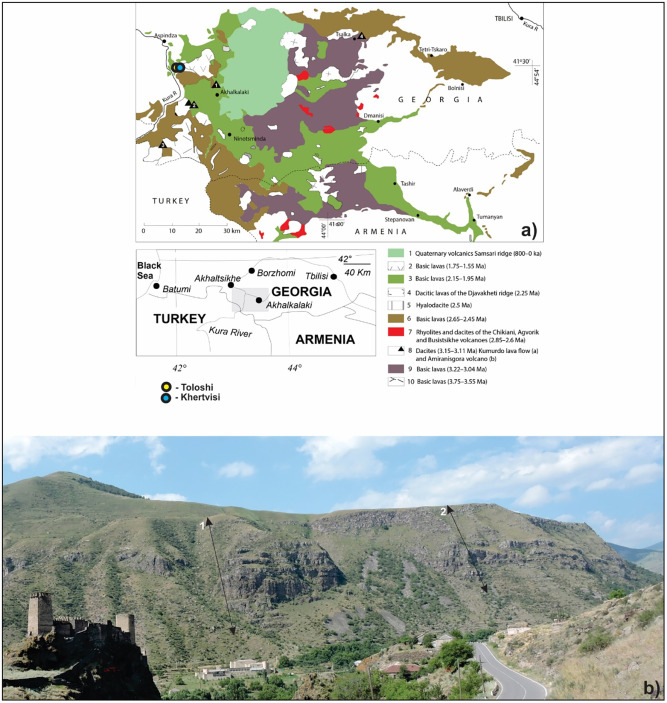
\includegraphics[width=12cm]{2.jpg}
    \caption{Schematic geological map of the Pliocene-Pleistocene magmatism in the Javakheti Highland showing the location of the Toloshi (1) and Khertvisi (2) sections
(modified after Lebedev et al., 2008). Paleomagnetic data from Toloshi profile are reported in Goguitchaichvili et al., 2021 while Khertvisi lava succession denote to
present study (see text for more details).
1 - Late Quaternary volcanic rocks (andesites and dacites) of the Samsari ridge (<800 ka); 2–10 Pliocene – Early Quaternary volcanic rocks of the Akhalkalaki
Formation (2 - basic lavas 1.75–1.50 Ma, 3 - basic lavas 2.15–1.95 Ma, 4 - later dacites and rhyolites of the Javakheti ridge 2.25 Ma, 5 - hyalodacite 2.5 Ma, 6 - basic
lavas 2.65–2.45 Ma, 7 - earlier rhyolites and dacites of the Javakheti ridge 2.85–2.6 Ma, 8 - dacites of the SW part of the Javakheti highland 3.15–3.11 Ma, 9 - basic
lavas 3.22–3.04 Ma, 10 - basic lavas 3.75–3.55 Ma). Also shown is a simplified stratigraphic diagram showing the thicknesses of 20 consecutive lava flows.}
    \label{fig:my_label}
\end{figure}


Still, the precise estimation of the top and base of the Olduvai subchron is a matter of debate (Channell et al., 2020). After Shackleton et al. Physics of the Earth and Planetary Interiors 333 (2022) 106952
2(1990), the base of Olduvai corresponds to an age of 1950 ka. The same conclusion was reached by Hilgen in 1991 (see also Lourens et al., 1996and Ogg, 2012). Lisiecki and Raymo (2005) suggested the base of Olduvai at 1968 ka, while Rivera et al. (2017) place it at 1948 ± 2 ka based on an 40Ar/39Ar age determination. As far as the uppermost Olduvai age is concerned, the most comprehensive study belongs to Singer (2014), suggesting an age of 1787 ± 15 ka for the top of the Olduvai based on isotopic dates.
\\
There is a general agreement among the paleomagnetic community
that the Olduvai subchron is characterized by normal polarity magne-
tization. Numerous studies showed, however, that the whole subchron is
probably not uniform. Intermediate polarity lava flows were reported by
Singer and Laurie (2004), while Tric et al. (1991) found a transitional
field in marine sediments. A short inverted polarity, within the Olduvai
event, was reported by Zijderveld et al. (1991), Yang et al. (2008), and
Kusu et al. (2016). Goguitchaichvili et al. (2021) reported a detailed
rock-magnetic and paleomagnetic study of the Lesser Caucasus lava
sequence at Toloshi, comprised between 1.93 ± 0.09 and 1.78 ± 0.11
Ma. All twenty lava flows yielded clearly defined reverse polarity
magnetization interpreted as a relatively short geomagnetic event
within the normal-polarity Olduvai subchron. Because of the importance
of these findings, additional samples were collected from a nearby,
parallel Khertvisi section comprised of 21 consecutive lava flows. Both,
new isotopic ages and paleomagnetic results were obtained. In addition,
multi-specimen absolute intensity determinations were successfully
determined for five independent cooling units.
\begin{figure}
    \centering
    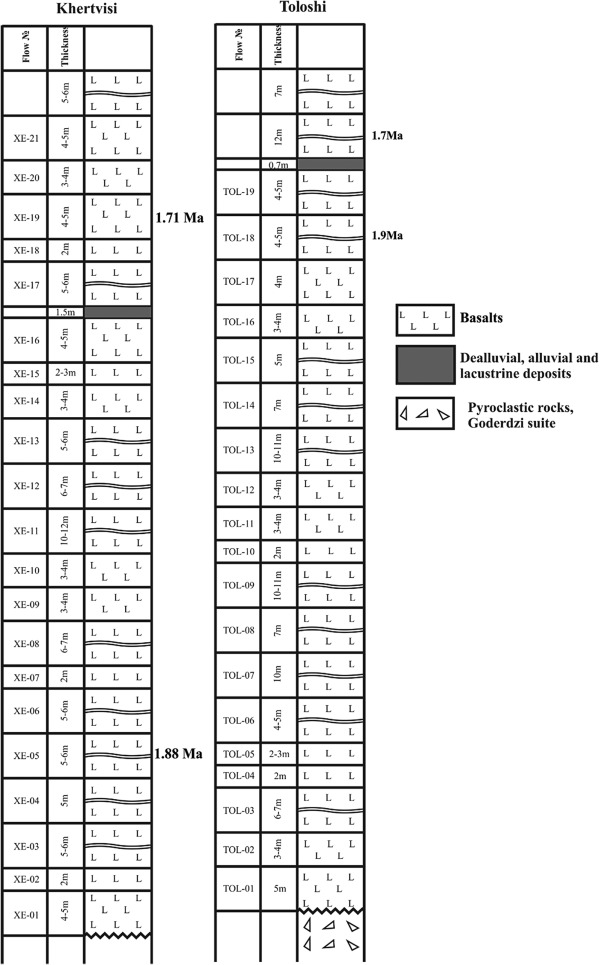
\includegraphics{3.jpg}
    \caption{A simplified stratigraphycal column for Khertvisi and Toloshi sections. See text for more details.}
    \label{fig:my_label}
\end{figure}
\begin{table}[h!]
    \centering
    \caption{Isotopic age determinations for two Khertvisi lava flows. Please see text for technical details.}
    \resizebox{\linewidth}{!}{
    \begin{tabular}{c|c|c|c|c|c|c}
    Lab Code & Rock type & Object & $K, \% \pm \sigma$ & $^{40}Ar^* \pm \sigma$ & $^{40}Ar_{atm},\%(in sample)$ & Age, Ma $\pm 2\sigma$\\
    \hline
         XE-19 & Basalt & Khertvisi, Upper Part & $0.77 \pm 0.015$ & $0.091 \pm 0.002$ & 59.5 & $1.71 \pm 0.10$  \\
         XE-05 & Basalt & Khertvisi, Lower Part & $0.95 \pm 0.015$ & $0.124 \pm 0.003$ & 91.6 & $1.88 \pm 0.12$ 
    \end{tabular}
    }
    \label{tab:my_label}
\end{table}
\\
New radiometric ages obtained in this study were performed in the
Institute of Geology of Ore Deposits, Petrography, Mineralogy, and
Geochemistry – Russian Academy of Sciences. The methodology is the
same as the one used in Goguitchaichvili et al. (2021). The microlithic
groundmass of lavas separated from phenocrysts was used for the
dating. The analyses of radiogenic 40Ar content were carried out on the
high-sensitive low-blank mass spectrometer MI-1201 IG (SELMI) (Leb-
edev et al., 2010). The isotopic dilution technique with monoisotopic
38Ar as spike was used. Correctness of measurements was controlled by
repeating analyses of the international standard samples MMhb-1, Bern-
4 M, muscovite P-207, and argon with atmospheric composition. The
total blank of 40Ar in analyses did not exceed 0.003 ng. The potassium
content of the samples was determined by the flame photometry method
using an FPA-01 spectrometer (ELAM Center). The total uncertainties of
K-Ar dating (±2$\sigma$) are given in Table 1, together with age values. The
calculations were based on the international values of decay constants
for radioactive isotopes (Steiger and J{\"a}ger, 1977).

\section{Sampling details and isotopic dating}
The studied area belongs to the Javakheti Highland, characterized by
an extremely intense Pliocene-Quaternary volcanic activity in the
northwestern sector of the Lesser Caucasus (Fig. 1a). Some details con-
cerning regional geology and the evolution of young magmatism were
discussed (Lebedev et al., 2008, 2019). A brief geological description of
the studied area (northwestern part of Javakheti Highland near the
confluence of rivers Mtkvari and Paravani is given in Goguitchaichvili
et al. (2021). In this study, we sampled a Khertvisi lava sequence, which
represents a parallel section (Fig. 1b) to the previously analyzed Toloshi
sequence (Goguitchaichvili et al., 2021). Both sites are located on the
left bank of the Mtkvari (Kura) River (Fig. 2). The Khertvisi sequence
comprises twenty-one lava flows of calc-alkaline basalts
(SiO2–48.7–50.7, Na2O + K2O – 4.7, K2O – 1.0–1.1 wt\%) with variable
thicknesses from about 2 to 10 m. A 1.5 m thick reddish sedimentary
layer is detected between lava flows XE16 and XE17. The same layer is
only half thick in the Toloshi section. In any case, the existence of such a
unit reflects some kind of interruption of lava emission dynamics. At least eight standard paleomagnetic cores were collected and oriented
with both magnetic and sun compasses in each flow. In a few cases, the
solar orientation was impossible, and the local declination value was
used as a correction factor. No tectonic correction was applied since no
significant or measurable dip was observed during the fieldwork.

\section{Magnetic measurements} 
Continuous thermomagnetic curves (susceptibility vs. temperature)
were recorded up to 600 $^{\circ}$C using an AGICO MFK1a Kappabridge with a
heating (and cooling) rate held to 15 $^{\circ}$C per minute. The experiments
were performed in argon to avoid potential magneto-chemical changes.
These measurements (Fig. 3) are useful to estimate the thermal stability determinations, as well as to reveal magnetic carriers through the determination of their Curie points.
\\
\begin{figure}
    \centering
    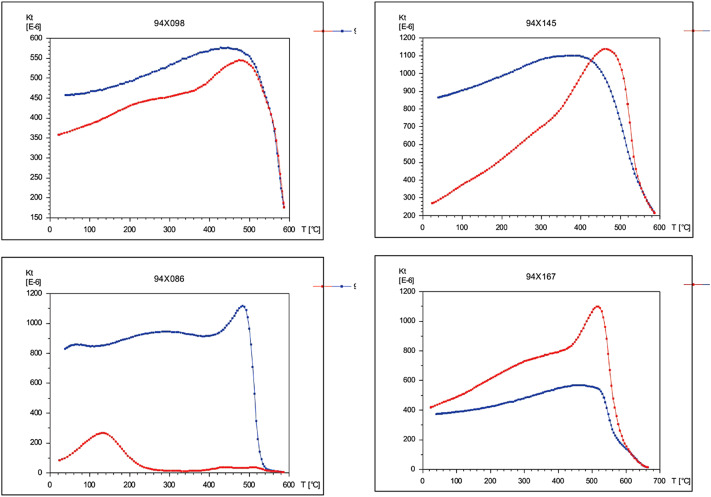
\includegraphics[width=12cm]{4.jpg}
    \caption{Representative examples of magnetic susceptibility vs. temperature curves. The red and blue lines indicate the behavior during heating and cooling
respectively, the relative susceptibility is shown in arbitrary units. (For interpretation of the references to colour in this figure legend, the reader is referred to the web
version of this article.)}
    \label{fig:my_label}
\end{figure}
\begin{figure}
    \centering
    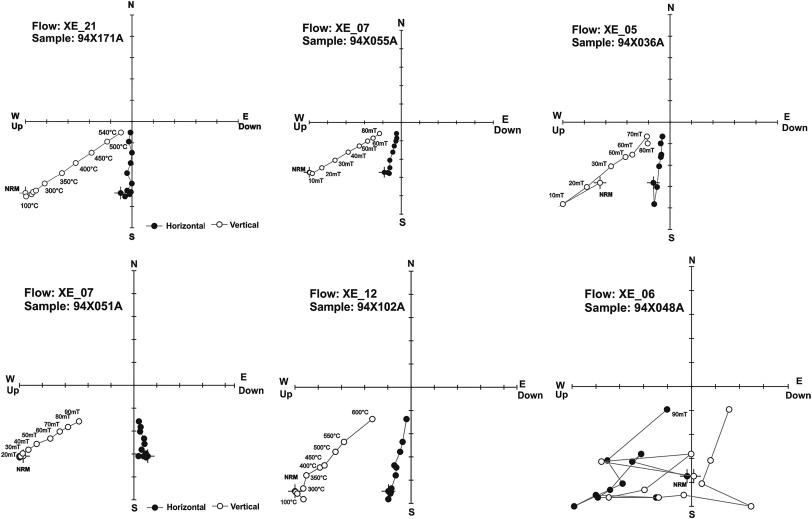
\includegraphics[width=12cm]{5.jpg}
    \caption{Orthogonal demagnetization vector plots for representative samples. The numbers refer to the peak values of alternating fields expressed in mT or degrees
Celsius for the maximum temperature value step.}
    \label{fig:my_label}
\end{figure}
\begin{figure}
    \centering
    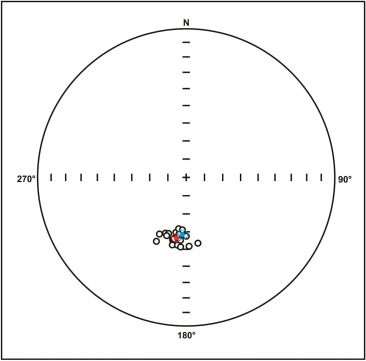
\includegraphics{6.jpg}
    \caption{Flow-mean characteristic paleodirections for the Khertvisi lava flows.
The red circle is the mean direction and his 95\% confidence for this study, circle
in blue is the direction retrieved from APTW for Eurasia for the last 5 Ma (Besse
and Courtillot, 2002). (For interpretation of the references to colour in this
figure legend, the reader is referred to the web version of this article.)}
    \label{fig:my_label}
\end{figure}
\begin{figure}
    \centering
    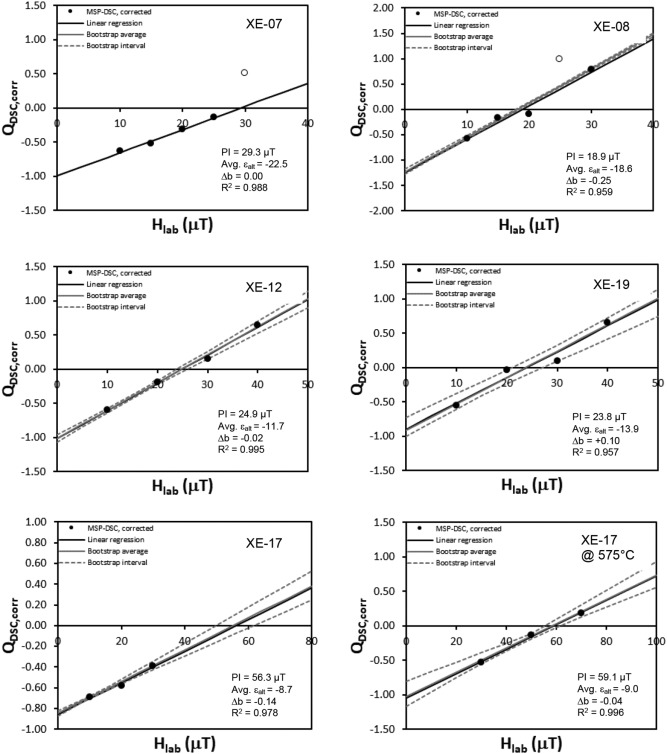
\includegraphics[width=12cm]{7.jpg}
    \caption{Representative examples of multi-specimen absolute intensity determinations using the MSP-VBA Tool (Monster et al., 2015). 475 $^{\circ}$C was used for all samples
to produce partial thermoremanences except flow XE-17, which was additionally subjected to 525 $^{\circ}$C. Please see the text for more details.}
    \label{fig:my_label}
\end{figure}
To determine flow-mean paleodirections (Fig. 4 and 5), eight speci-
mens per flow, on average, were subjected to either alternating field
demagnetization using an LDA-3 AGICO demagnetizer up to 90 mT, or
thermal treatments until 600 ◦C (Fig. 4) using an MMTD80 device. At
least six aligned steps pointing to the origin were used to calculate
inclination and declination at the sample level, with values of maximum
angular deviation less than 3◦. The remanence components were
determined using the principal component analysis method (Kirschvink,
1980), while the determination of flow-mean paleodirections was based
on the Fisher statistics (Fisher, 1953).
\\
Absolute paleointensity determinations were carried out with the
multispecimen parallel differential pTRM method (Dekkers and B{\"o}hnel,
2006), including the protocols for fraction and domain-state corrections
(FC, DSC, respectively) (Fabian and Leonhardt, 2010), hereafter referred
as MSP. The specimen preparation for the MSP was as follows: One
standard paleomagnetic core per flow was cut into two disc-shaped
halves; each of them was further split into pie-slices-shaped quarters,
obtaining eight sub-specimens in total. Each sub-specimen was pressed
into a salt pellet with standard paleomagnetic dimensions. Based on AF
demagnetization plots of pilot specimens, which revealed the presence
of small secondary imprints, a 5 mT demagnetization was applied to the
sub-specimens before applying the MSP in order to eliminate possible
viscous overprints.
\\
The MSP experimental protocol (Fig. 6) consisted of the sequence of
the following steps: (a) measurement of the NRM vector; (b) using a
special ten-position sample holder, specimens were oriented in such a
way that the NRM directions of each sub-specimen lay parallel to the
heating chamber axis; subsequently they were heated at the corresponding temperature in an axial laboratory field and therefore
parallel to the remanence of the specimens(see below); (c) specimens
were set and heated as in the previous step but in an anti-parallel field;
(d) specimens were heated in zero-field and cooled in a parallel labo-
ratory field; (e) step (b) was repeated. After each of the steps (b) to (e),
the acquired magnetization was measured using an AGICO JR6 spinner
magnetometer. As stated by Monster et al. (2015), the QDB ratio
(Dekkers and B{\"o}hnel, 2006) is defined as follows:
\\
$$
Q_{DB}=\frac{m_1-m_0}{m_0}
$$
where $m_0$ and $m_1$ are the scalar intensities of the two remanences. The fraction-corrected (MSP-FC) and domain-state corrected (MSP-DSC) ratios (both defined in Fabian and Leonhardt, 2010) are:
$$
Q_{FC}=2*\frac{m_1-m_0}{2m_0-m_1-m_2}
$$
$$
Q_{DSC}=2*\frac{(1+\alpha)m_1-m_0-\alpha m_3}{2m_0-m_1-m_2}
$$
Based on the Curie temperatures estimated from K-T curves, a temperature of 475 $^{\circ}$C was used for the different heatings. This temperature is low enough to reduce the risk of thermal alteration of the magnetic mineralogy but sufficient to create a significant partial thermoremanence. Experiments were performed using an ASC Scientific TD48-SC furnace.
\\
A set of laboratory fields ranging from 20 to 70 $\mu T$ was applied to the
different sub-specimens, initiating at 20 $\mu T$, and increasing its value
until the QDB ratio (Dekkers and B{\"o}hnel, 2006) plotted above the horizontal zero value. When possible, the experimental procedure was repeated to get an equal number of points below and above the horizontal line. All calculations were performed using the VBA software of Monster et al. (2015). Exceptionally, the entire MSP was repeated at a higher temperature of 525 $^{\circ}$C for the sample XE-17 (see the details below).
\section{Main results}
Most of the studied lava flows exhibited irreversible susceptibility vs
temperature behavior during the heating and cooling cycles (Fig. 3),
similar to the Toloshi lava flows (Goguitchaichvili et al., 2021). Two
ferromagnetic phases seem to be present in the third part of the flows
(see an example in Figure3, Sample 95 × 086). A relatively low Curie
temperature is observed between 180 and 190 ◦C, while a High-T phase
is detected around 550 ◦C, which most probably corresponds to some
Titanium poor titanomagnetites. The Curie points, determined for the
remaining samples range between 558 and 576 ◦C, which again attest to
the presence of almost magnetite phases. The irreversibility, and thus
thermal instability observed for the majority of samples, seems to be
produced at high temperatures, close to the blocking temperature
spectra.
Magnetic treatments permitted the precise determination of flow-
mean paleodirections for all cases, except for site XE06 (sample
94X048A in Fig. 4). The chaotic and unstable demagnetization behavior
impeded selecting any linear segment going to the origin. For all other
flows, both thermal and alternating field treatments showed great efficiency revealing essentially univectorial component magnetization.
Viscous remanence is almost inexistent or easily removed at the very
first steps of the magnetic cleanings. Similar to Toloshi’s (Goguitch-
aichvili et al., 2021), all Khertvisi lava flows yielded a well-defined
reverse polarity magnetization, which is very precisely determined
(Fig. 5, Table 2) judging from the precision parameter values of the
Fisher statistics.
The mean direction, involving all accepted flows, is Inc. = $-56.1^{\circ}$, Dec=$189.5^{\circ}$, $N=20$, $\alpha_{95}=2.3^{\circ}$, k=187. These directions are close to
the Toloshi’s mean paleodirections, and both slightly deviate clockwise
from the geocentric axial dipole direction and the expected directions
recalculated from the stable Eurasia reference paleomagnetic poles
(Besse and Courtillot, 2002). We do not believe that this declination
deviation is due to some tectonic movements since the duration of lava emissions apparently happened during a very short time and thus, the
secular variation is most probably not averaged. Secular variation parameters ($S_b=7.8^{\circ}$ with upper limit $S_{bu}=8.5^{\circ}$ and lower limit $S_{bl}=7.1^{\circ}$) calculated through virtual geomagnetic pole scatter (Cox, 1970) yielded very low values compared to the available models (Tauxe and
Kent, 2004).
\\
As multispecimen paleointensity determinations are concerned (Fig. 6), the reliability criteria applied for the MSP relied on the two reliability checks provided by the MSP-Tool of Monster et al. (2015): the average alteration parameter (Avg. $\epsilon_{alt}$) and the difference between the theoretical and experimental intersection with the y axis ($\Delta b$), since, as mentioned by Monster et al. (2015), “Alteration, domain-state effects or alignment errors, however, may lead to a different intercept”. An Avg.  $\epsilon_{alt} \leq 20\%$  (Carvallo et al., 2017) was set in this investigation. Additionally, a negative overprint check, i.e. $\Delta dec$ $(\Delta inc) < 15^{\circ}$ (Monster et al., 2015) was required.
\\
Three out of the six analyzed flows (XE-07, XE-12, and XE-19) yielded successful domain state corrected (DSCc, Monster et al., 2015) paleointensity determinations with values between 23.8  $\mu T$ and 29.3  $\mu T$, which are at least 50\% lower than the present-field value. Flows XE-08 and XE-17 failed to accomplish the $\Delta b$ reliability check, while flow XE-15 produced no reliable results at all. Moreover, flow XE-17 yielded a higher DSCc field value of 56.3 $\mu T$. Worth noting is the fact that, despite the low chosen heating temperature of $475^{\circ}$, Avg $\epsilon_{alt}$ range is between 8.7 and 22.5\%.
\\
We also note that the \%NRM lost values for flows XE-15 and XE-17 obtained during the MSP carried out at a temperature of $475^{\circ}$ were at the most 23\% and 34\%, respectively; which are likely low enough to
be considered as a suitable pTRMs for reliable determination. Therefore, for these two flows, we decided to repeat the entire MSP but at a higher temperature. This approach seems to be adequate since the Avg $\epsilon_{alt}$ obtained for these flows was well below the threshold value of 20\%, and all the specimens will experience again the same thermal history. Thus, the entire MSP was repeated for these flows at a temperature of $525^{\circ}$. This time, the \%NRM lost values obtained for flow XE-17 was 50\% on average, and yielded a slightly higher DSCc field value of 59.1 $\mu T$, with an Avg $\epsilon_{alt}$ of 9\% and fulfilling the reliability criteria established. It is highly encouraging that both measurements yielded very similar values. Again, flow XE-15 failed to provide any reliable paleointensity determination. Detailed results -Min and Max PI values, $\Delta b$, and Avg $\epsilon_{alt}$ values, including the other ratios (DBc and FCc)- can be consulted in Table 3.
\section{Discussion and conclusions}
The new isotopic age determinations indicate that the lavas of the Khertvisi section erupted in the Early Pleistocene, at the boundary of the Gelasian and Calabrian ages in a time span of 1.88 to 1.71 Ma; in good
agreement with the Toloshi lava sequence (1.93–1.78 Ma). Although a sedimentary layer is observed in both sections, the duration of the lava emissions seems to be very short – unable to average paleosecular
variation. All studied lava flows yielded reverse polarity magnetization, while mean paleodirections are slightly deviated (clockwise) from the axial dipole and expected directions. The upper part of the sequence (few lava flows) above the reddish sedimentary layer may be alternatively correlated to Chron C1r.3r in the geomagnetic polarity time scale, and the lower part (the great majority of lava flows) below the
mentioned layer to Chron C2r.1r. This approach suggests that the whole Olduvai subchron is completely missing in both Khertvisi (this study) and Toloshi (Goguitchaichvili et al., 2021) profiles. However, this
alternative correlation is probably untenable because of the following: 1) It appears that most consecutive (sequential) flows of the Khertvisi sequence show undistinguishable palaeomagnetic directions. For this
reason, and in order to analyze the characteristics of secular variation recorded in the sequence, several directional groups (DG) may be defined. If the 95\% confidence ovals of the directions of two consecutive
flows did not overlap, both directions are considered to be different. This procedure was systematically applied (see for instance Goguitchaichvili et al., 2009 and Caccavari et al., 2014) to the Javakheti lava sequences (see also Goguitchaichvili et al., 2021). However, in the present case, the scatter of individual VGP directions is extremely low and lavas above and below the reddish sedimentary layer show statistically undistinguishable paleodirections, indicating that all flows were emitted in a very narrow age interval; 2) The Olduvai normal subchron is not uniform and still no consensus exists on the duration and length. This is
perfectly illustrated by listing major paleomagnetic and associated geochronology works in Goguitchaichvili et al., 2021. Namely, many previous studies based on high-quality supported isotopic data, persistently reveal reverse polarity short-lived events within the Olduvai subchron.
\\
Besides great efforts during the last few decades, reliable paleointensity data are still insufficient to document a long-term variation in the intensity of the Earth’s magnetic field. A major reason for this
paucity is that absolute paleointensity is the most difficult component of the geomagnetic field to determine, and the laboratory experiment failure rate is generally 80 or even higher for volcanic rocks. Even though high-quality Thellier paleointensity determinations are obtained, their interpretation in terms of geomagnetic significance is complex (Calvo et al., 2002). Judging from continuous thermomagnetic
curves, it is clear that Khertvisi samples are unsuitable for Thellier double heating paleointensity experiments. In this study, paleointensity determinations were accomplished with the multispecimen parallel
differential pTRM method (Dekkers and B{\"o}hnel, 2006), together with the protocols for fraction and domain-state corrections (FC and DSC, respectively) proposed by Fabian and Leonhardt (2010) meeting most strict selection and quality criteria. In this context, five new, technically high-quality determinations should be considered as an absolute success.
\\
Goguitchaichvili et al. (2000) reported a reconnaissance study in three volcanic provinces in Georgia, Kazbegi, Kharmi, and Djavakheti (Camps et al., 1996; Calvo-Rathert et al., 2008 and 2015). This survey
also included the new evaluation of previous paleomagnetic results obtained by Sologashvili (1986) in an extensive paleomagnetic and magnetostratigraphic study carried out on more than a hundred lava flows from these three main Pliocene and Quaternary volcanic regions in Georgia. The absolute geomagnetic pleointensities obtained from Georgian volcanic units vary between 16.3 and 54.7 $\mu T$. It is worth
mentioning that two intermediate-polarity samples yield significantly reduced paleointensities (Calvo-Rathert et al., 2015). Discarding inter- mediate polarity sites, a mean value of a virtual dipole moment (VDM) of 7.8 ± 3.7 1022 Am2 is obtained close to the present-day value. Calvo-Rathert et al. (2011) analyzed more than 20 basaltic lava flows belonging to four different profiles in the southern Caucasus. Most flows yielded paleointensity results in the 30–45 $\mu T$ range, in accordance with expected Pliocene to present-day intensities. Two flows, however, yielded high paleointensity values around 60 $\mu T$. Goguitchaichvili et al. (2001) reported many successful Thellier type absolute geomagnetic paleointensity determinations from a Pleistocene lava sequence located in the Lesser Caucasus. Flow-mean Thellier paleointensity values range from 16.3 ± 5.2 to 71.0 ± 0.3 $\mu T$. The lowest values correspond to the transitional field regime and correspond to the Matuyama-Olduvai polarity transition.
\\
Four flows belonging to the Khertvisi profile yielded paleointensities ranging from 18.9 to 29.3 $\mu T$. Generally speaking, these values are close to transitional field intensities reported in Georgia during the Matuyama and Bruhnes chrons. One more Khertvisi flow provided higher paleointensity compared to the present-day field. Considering all these factors together, we definitively do not claim the existence of a transitional (geomagnetic reversal or excursion) field. However, high-quality paleomagnetic and absolute paleointensity data, supported by four isotopic ages and excellent stratigraphic control, most probably permit us to consider the Khertvisi section as the strong volcanic evidence of an unusual geomagnetic regime across the Olduvai subchron.
%%/////////////////////////////////////////////////////////////////////////////////////%%
%%/////////////////////////////////////////////////////////////////////////////////////%%
%%/////////////////////////////////////////////////////////////////////////////////////%%

%%/////////////////////////////////////////////////////////////////////////////////////%%
%%/////////////////////////////////////////////////////////////////////////////////////%%
%%/////////////////////////////////////////////////////////////////////////////////////%%
\section*{Author statement}
This study is headed by Avto Goguitchaichvili and Juan Morales. All authors actively participated either in field trips, laboratory experiments, interpretation and editing.

\section*{Declaration of Competing Interest}
We explicitely decalre that there is no conflict of interest.
\section*{Data availability}
Data will be made available on request.
\section*{Acknowledgments}
This work was funded by project PID2019-105796GB-100/ AEI/ 10.13039/ 501100011033 (Spanish Agencia Estatal de Investigac{\`i}on). This study was partially supported by the Natural Sciences and Engineering Research Council of Canada for V.A.K. (NSERC grant RGPIN-2019-04780). AG is gratefull to DGAPA-UNAM (Mexico) for the support during the sabbatical at University of Alberta).

*Because of there are so many references and linking to Google Scholar is difficult in mainland China, thus I just show 2 examples here to show my ability of editing by bib-file.
\\
Similarly, I just create ONE table to show my ability to make table.
\\
I would very appreciate it if your mightiness could give me a high score for my further study abroad. Thank you so much!

 Example1 \cite{Feynman1963118,Dirac1953888}.
 Example2 \cite{besse2002apparent}


\bibliography{mybibfile}

\end{document}